%!TEX root = ../../../thesis.tex
\begin{figure}
    \centering
    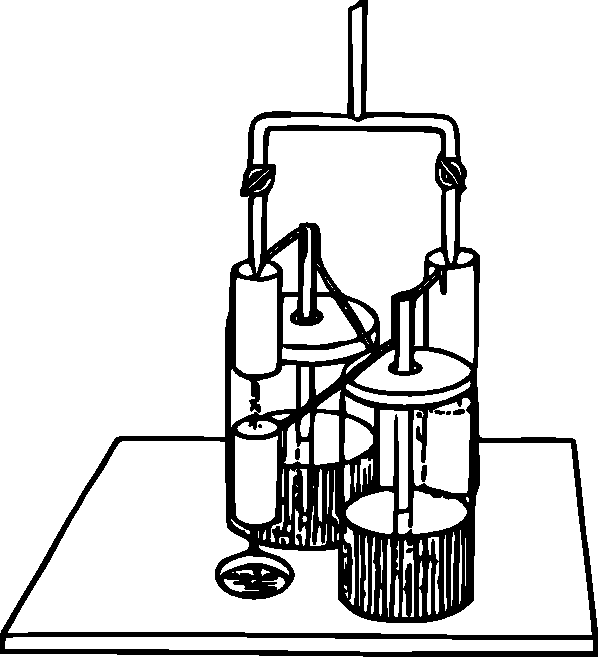
\includegraphics[width=0.5\textwidth]{content/appendices/chargedWaterDrops/graphics/Figure_Drawing_KelvinWaterDripper_OriginalDevice}
    \caption{Drawing of Lord Kelvin's electrostatic generator.}
    \label{Figure_Drawing_KelvinWaterDripper_OriginalDevice}
\end{figure}
In 1867 William Thomson (Lord Kelvin) described an apparatus that could generate electrostatic charge using drops of water (some of
which are shown in Figure \ref{Figure_Drawing_KelvinWaterDripper_OriginalDevice})
\cite{Thomson1867}.
This apparatus works by inducing charge onto drops of water before they detach from the source of the drips.
This device formed the basis for investigating the use of charged drops of water to generate useful amounts of power.


\section{Generating Charge}

\begin{figure}
    \centering
    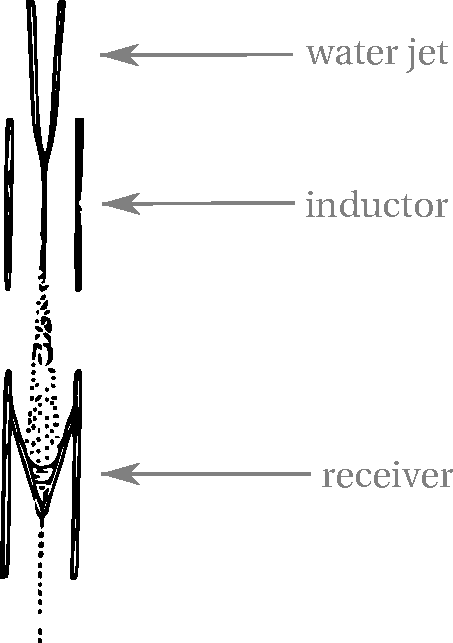
\includegraphics[height=0.25\textheight]{content/appendices/chargedWaterDrops/graphics/Figure_Drawing_KelvinWaterDripper_ChargingMechanism}
    \caption{Drawing of the charging mechanism for Lord Kelvin's electrostatic
generator}
    \label{Figure_Drawing_KelvinWaterDripper_ChargingMechanism}
\end{figure}
Figure \ref{Figure_Drawing_KelvinWaterDripper_ChargingMechanism} shows one of the charge generating mechanisms of Lord Kelvin's electrostatic generator.
This mechanism is comprised of three main components:
\begin{enumerate}
\item A jet of water which breaks into droplets
\item An inducting ring surrounding the area where the jet breaks up
\item A receiver where the charged droplets are collected
\end{enumerate}
A simplified diagram is shown in \cref{Fig_Diagram_KelvinWaterDripper}.
\begin{figure}
    \centering
    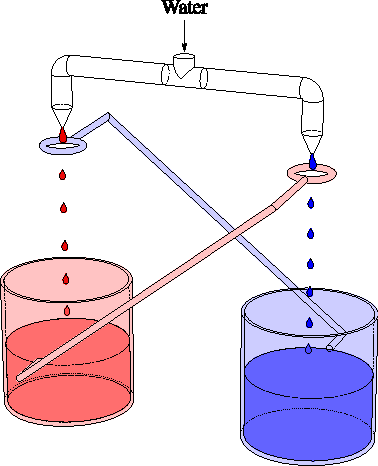
\includegraphics{content/appendices/chargedWaterDrops/graphics/DripperOut}
    \caption{\label{Fig_Diagram_KelvinWaterDripper}Simplified diagram of Lord Kelvin's water dropper configuration}
\end{figure}
The diagram illustrates the charge of each element by colour.
Equal and opposite amounts of electrical charge are accumulated in each container at the bottom.
These containers are electrically insulated from one another, but are connected to the rings (near the droppers) of the opposite side.
The rings are responsible for inducing excess charge on the drops.
They are the equivalent to the cylinder shaped inductor depicted in \cref{Figure_Drawing_KelvinWaterDripper_ChargingMechanism}).
Once detached, the drops are pulled by gravity into the containers below.
Because the container is already charged, there is a repulsive force between it and the falling drop.
It is this force acting over the distance through which the drop falls that does the work, further increasing the voltage of the container (and ring).

\section{Optimising output}

Summer research student Jonathon McMullen assembled a test-rig to recreate the experiment.
Once constructed, another summer research student, Wayne Crump, and myself took measurements.
Then we sought to optimise the design in the hopes that is may be suitable as an energy harvester.


\subsection*{Drop volume and frequency}

The first optimisation question in its most practical form was ``is it better to have lots of small drops or less larger drops?''.
To answer this question a more simplified experiment was performed with the help of another summer research student, Wayne Crump.
The purpose of this experiment was to remove as many variables from the electrostatic generator experiment performed by Jonathan McMullen.
The reason for doing this was to isolate the effect that varying drop size, induction voltage and flow rate had on the output.


 \subsubsection*{Experimental setup}

\begin{figure}
    \centering
    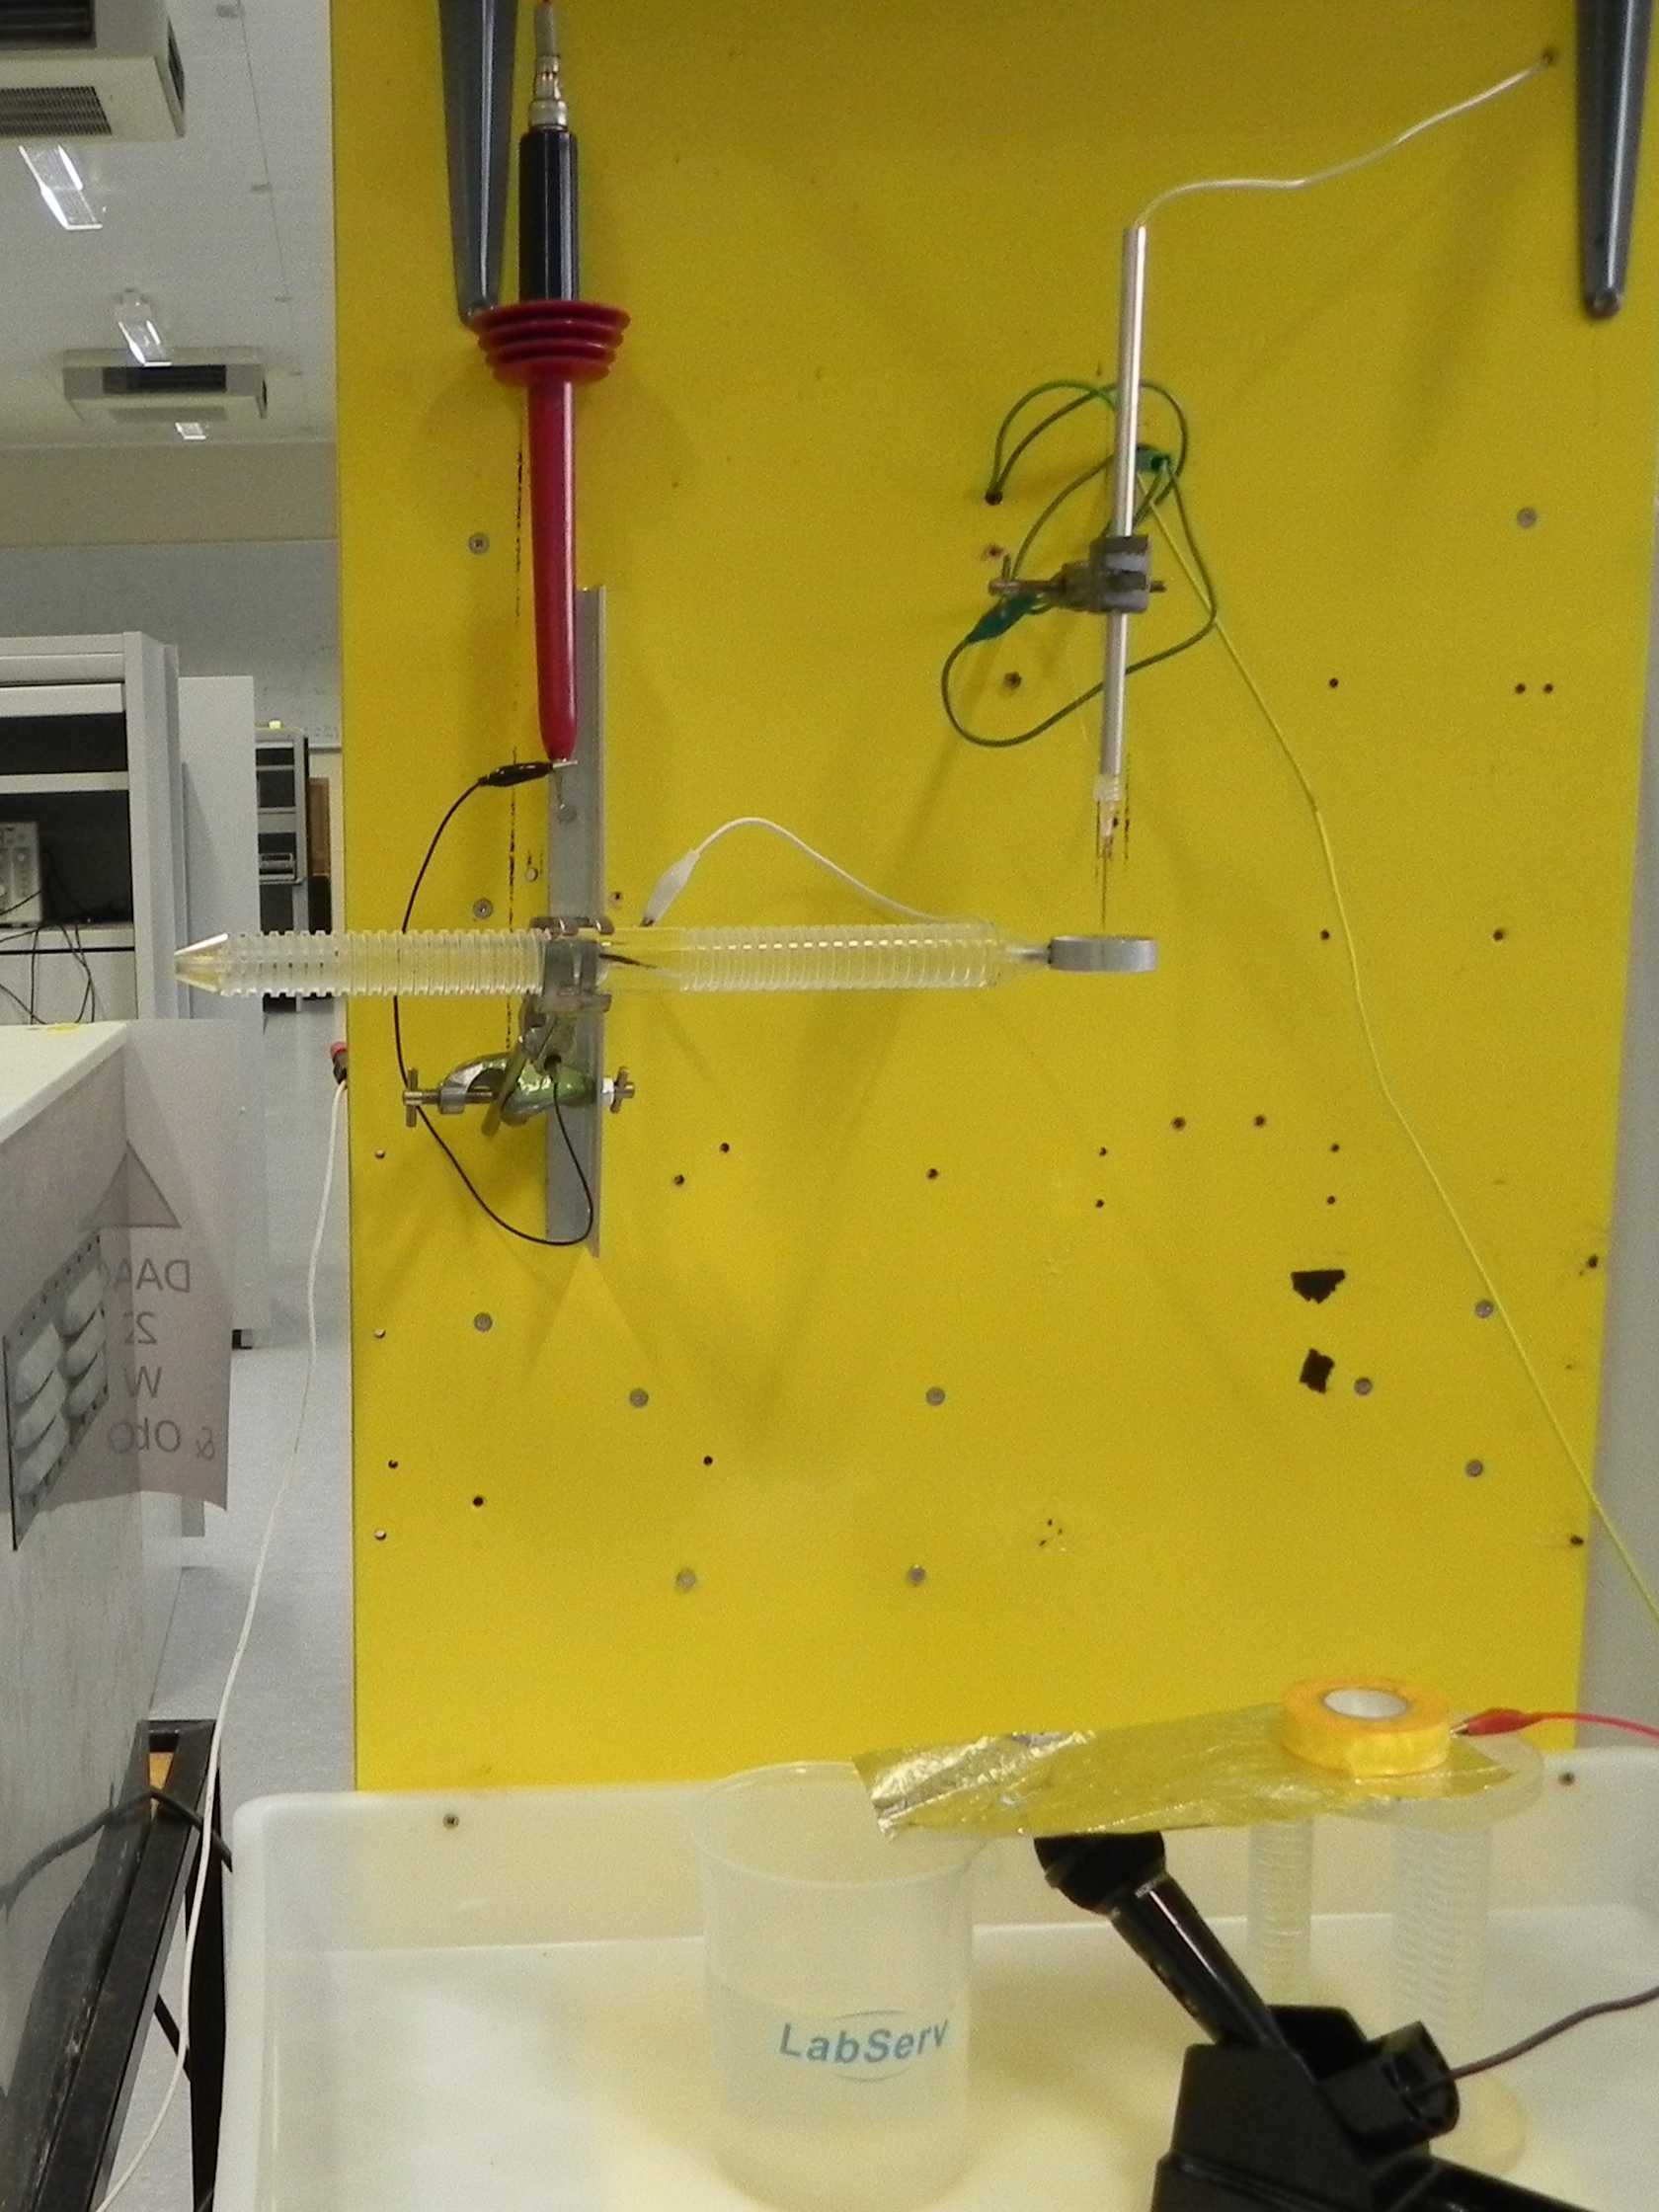
\includegraphics[scale=0.15]{content/appendices/chargedWaterDrops/graphics/Photo_dripperExperiment_Setup_draft.JPG}
    \caption{\label{Photo_dripperExperiment_Setup}Photo of experimental setup for charge on drip measurements.}
\end{figure}


A photo of the measurement setup can be seen in \cref{Photo_dripperExperiment_Setup}.
A simplified diagram of that setup is shown in \cref{ChargedDrips_Figure_Drawing_ExperimentalSetup}.
In this diagram, drips are formed from the end of a syringe needle, pass through the induction ring and land on a piece of tin foil before running off into a catchment container.
A close-up of view the needle and inductor is shown in \cref{Photo_dripperExperiment_Inductor}.
The frequency of drips is determined by microphone and the flow of water is set by the syringe pump (shown in \cref{Photo_dripperExperiment_SyringePump}).

\begin{figure}
    \centering
    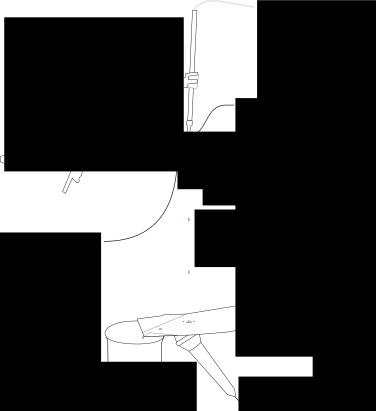
\includegraphics[scale=0.9]{content/appendices/chargedWaterDrops/graphics/ChargedDrips_Figure_Drawing_ExperimentalSetup}
    \caption{\label{ChargedDrips_Figure_Drawing_ExperimentalSetup}Diagram of experimental setup for charge on drip experiments.}
\end{figure}

The volume of each drip is calculate by dividing the flow rate by the drip frequency.
The charge on each drop of water was determined by dividing the average current by the drip frequency.
Drop size was determined by both the size of needle and the induction voltage placed on the ring.
Because the current being measured was so small (nano Amperes), direct measurement with a multimeter was not possible.
Instead the multimeter was set to measure voltage.
In this setting the multimeter has an internal resistance of \SI{10}{\mega\Omega} over which the voltage was being measured.
Ohms law states:

\begin{equation}
V=IR
\end{equation}
Where V is voltage, I is current and R is resistance.
Rearranging this equation and substituting in our resistance of \SI{10}{\mega\ohm} gives:

\begin{equation}
I=\frac{V}{10\times10^{6}}
\end{equation}
Where V is the output of the multimeter and I is the current through
the multimeter, through which we assume all charge collected on the
tin foil will flow.

\begin{figure}
    \centering
    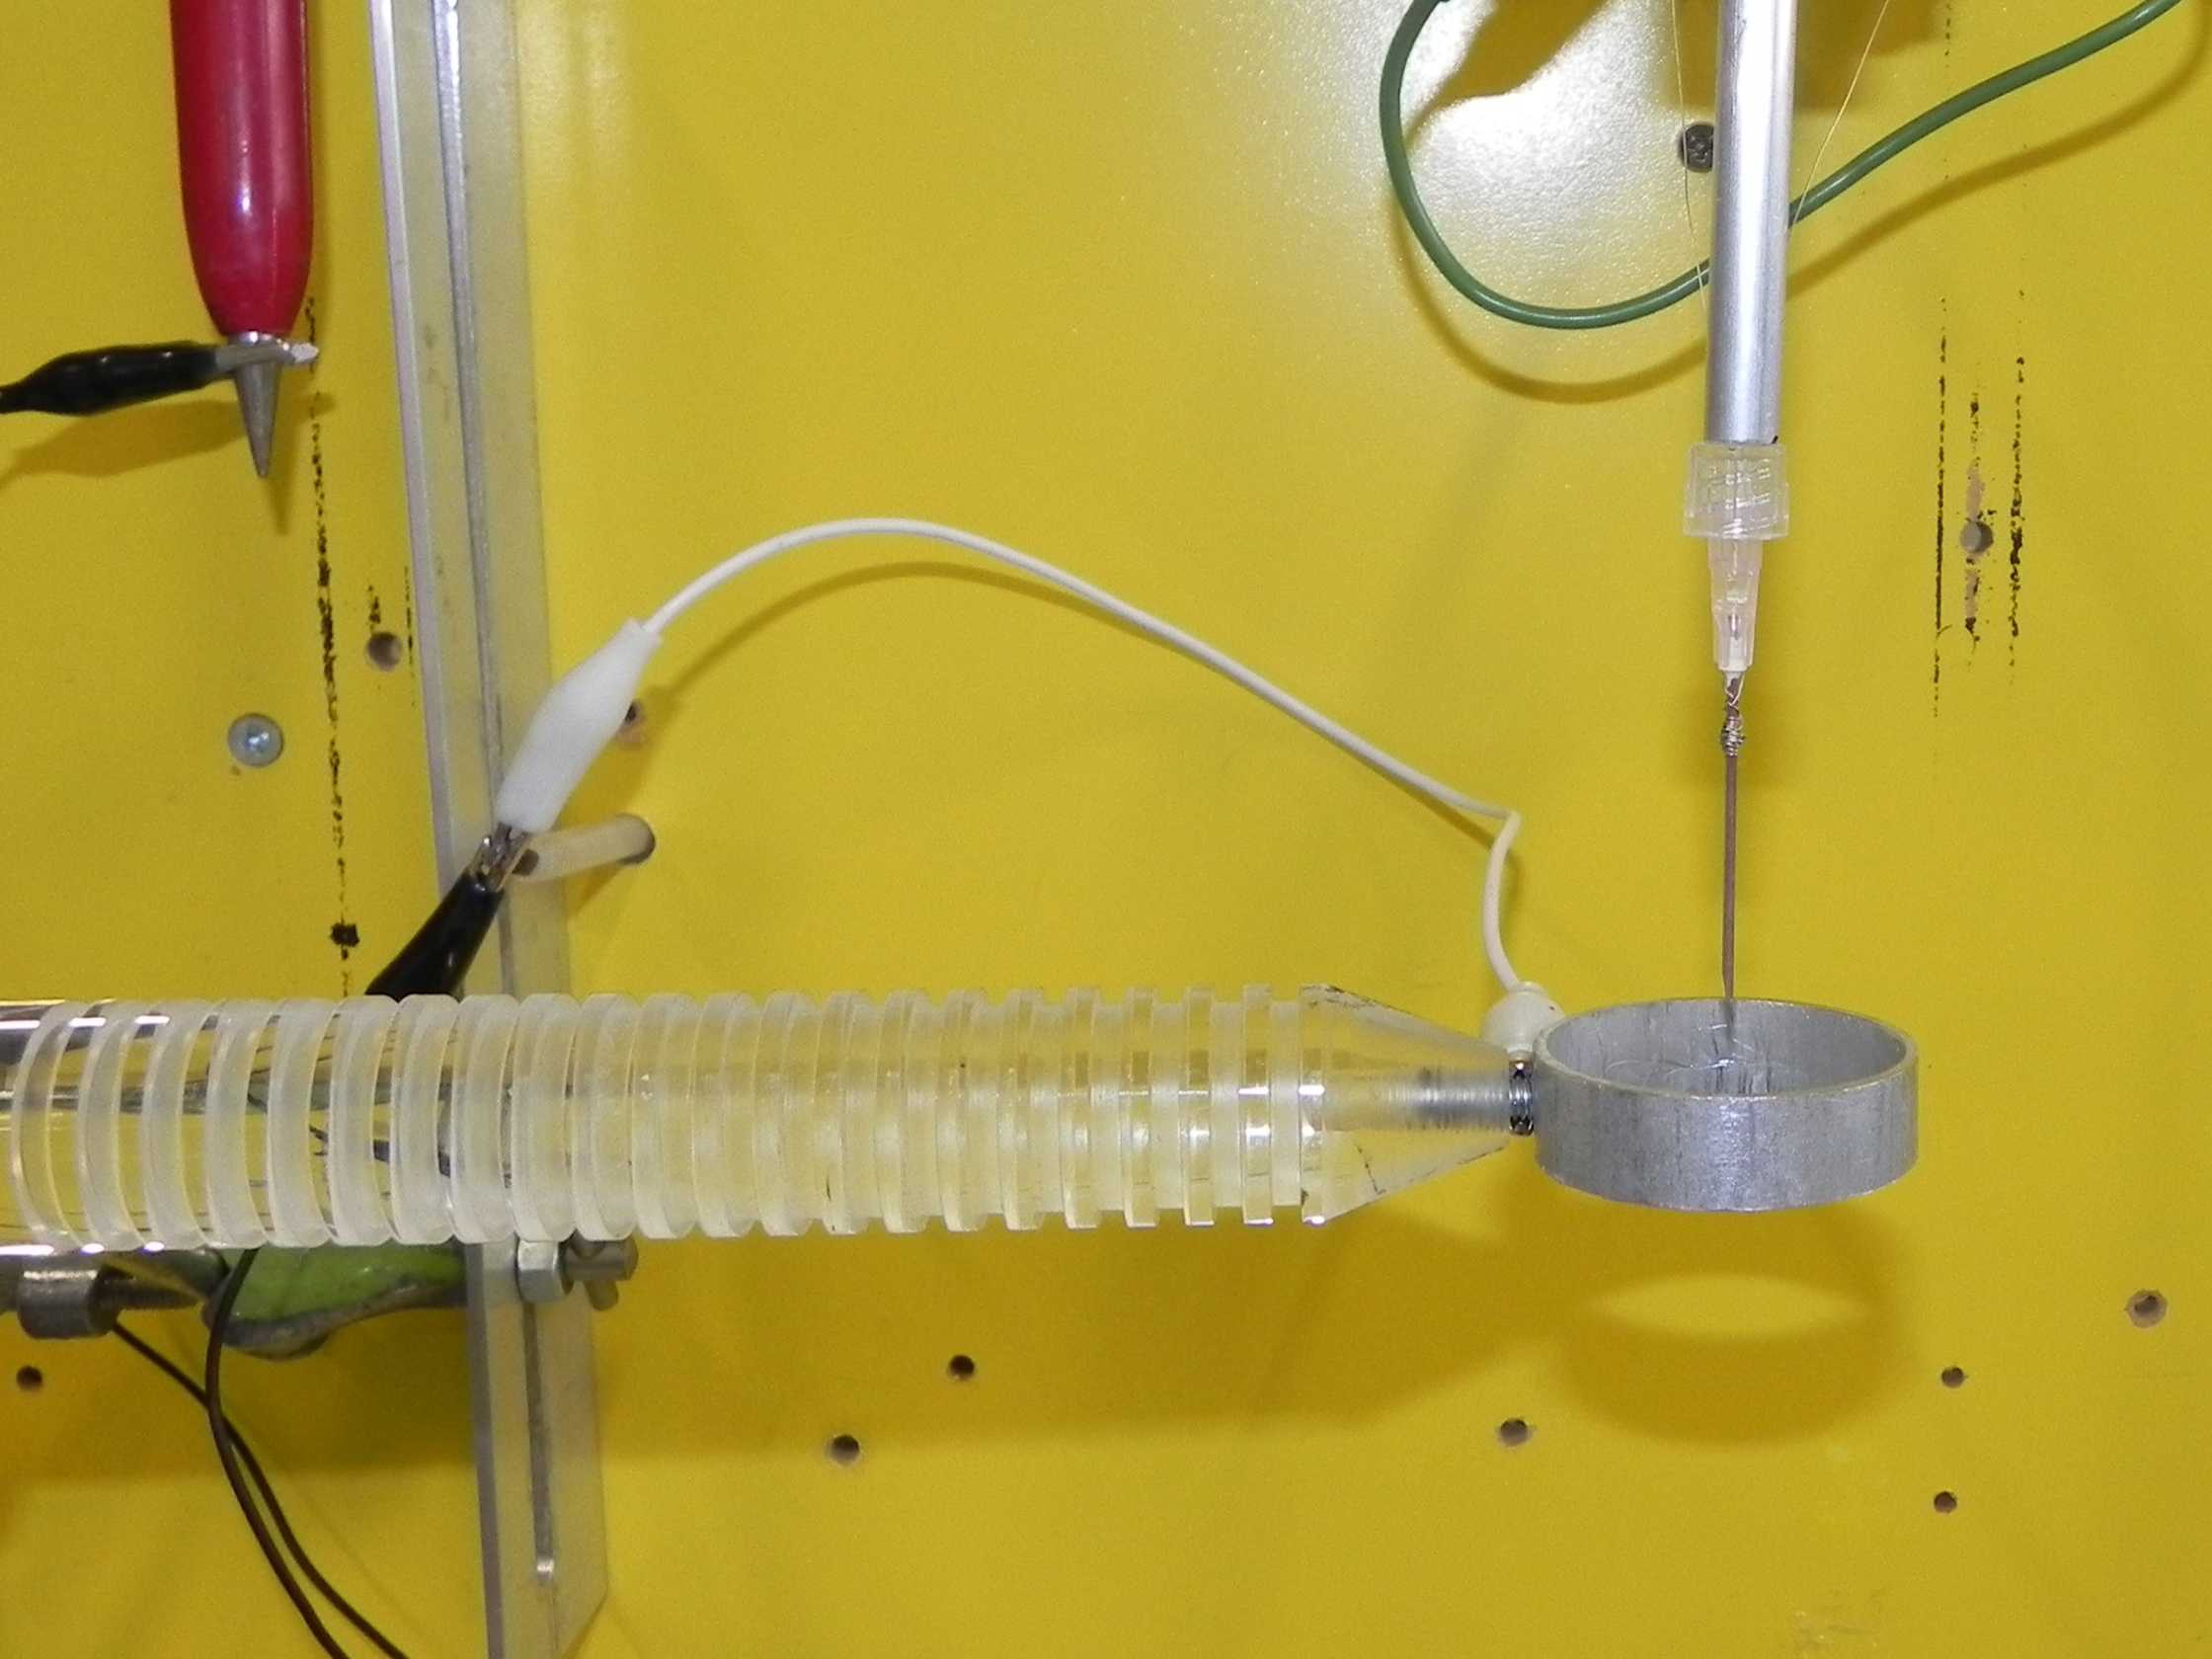
\includegraphics[scale=0.15]{content/appendices/chargedWaterDrops/graphics/Photo_dripperExperiment_Inductor_draft.JPG}
    \caption{Photo of the dropper and high voltage inductor.}
    \label{Photo_dripperExperiment_Inductor}
\end{figure}

\begin{figure}
    \centering
    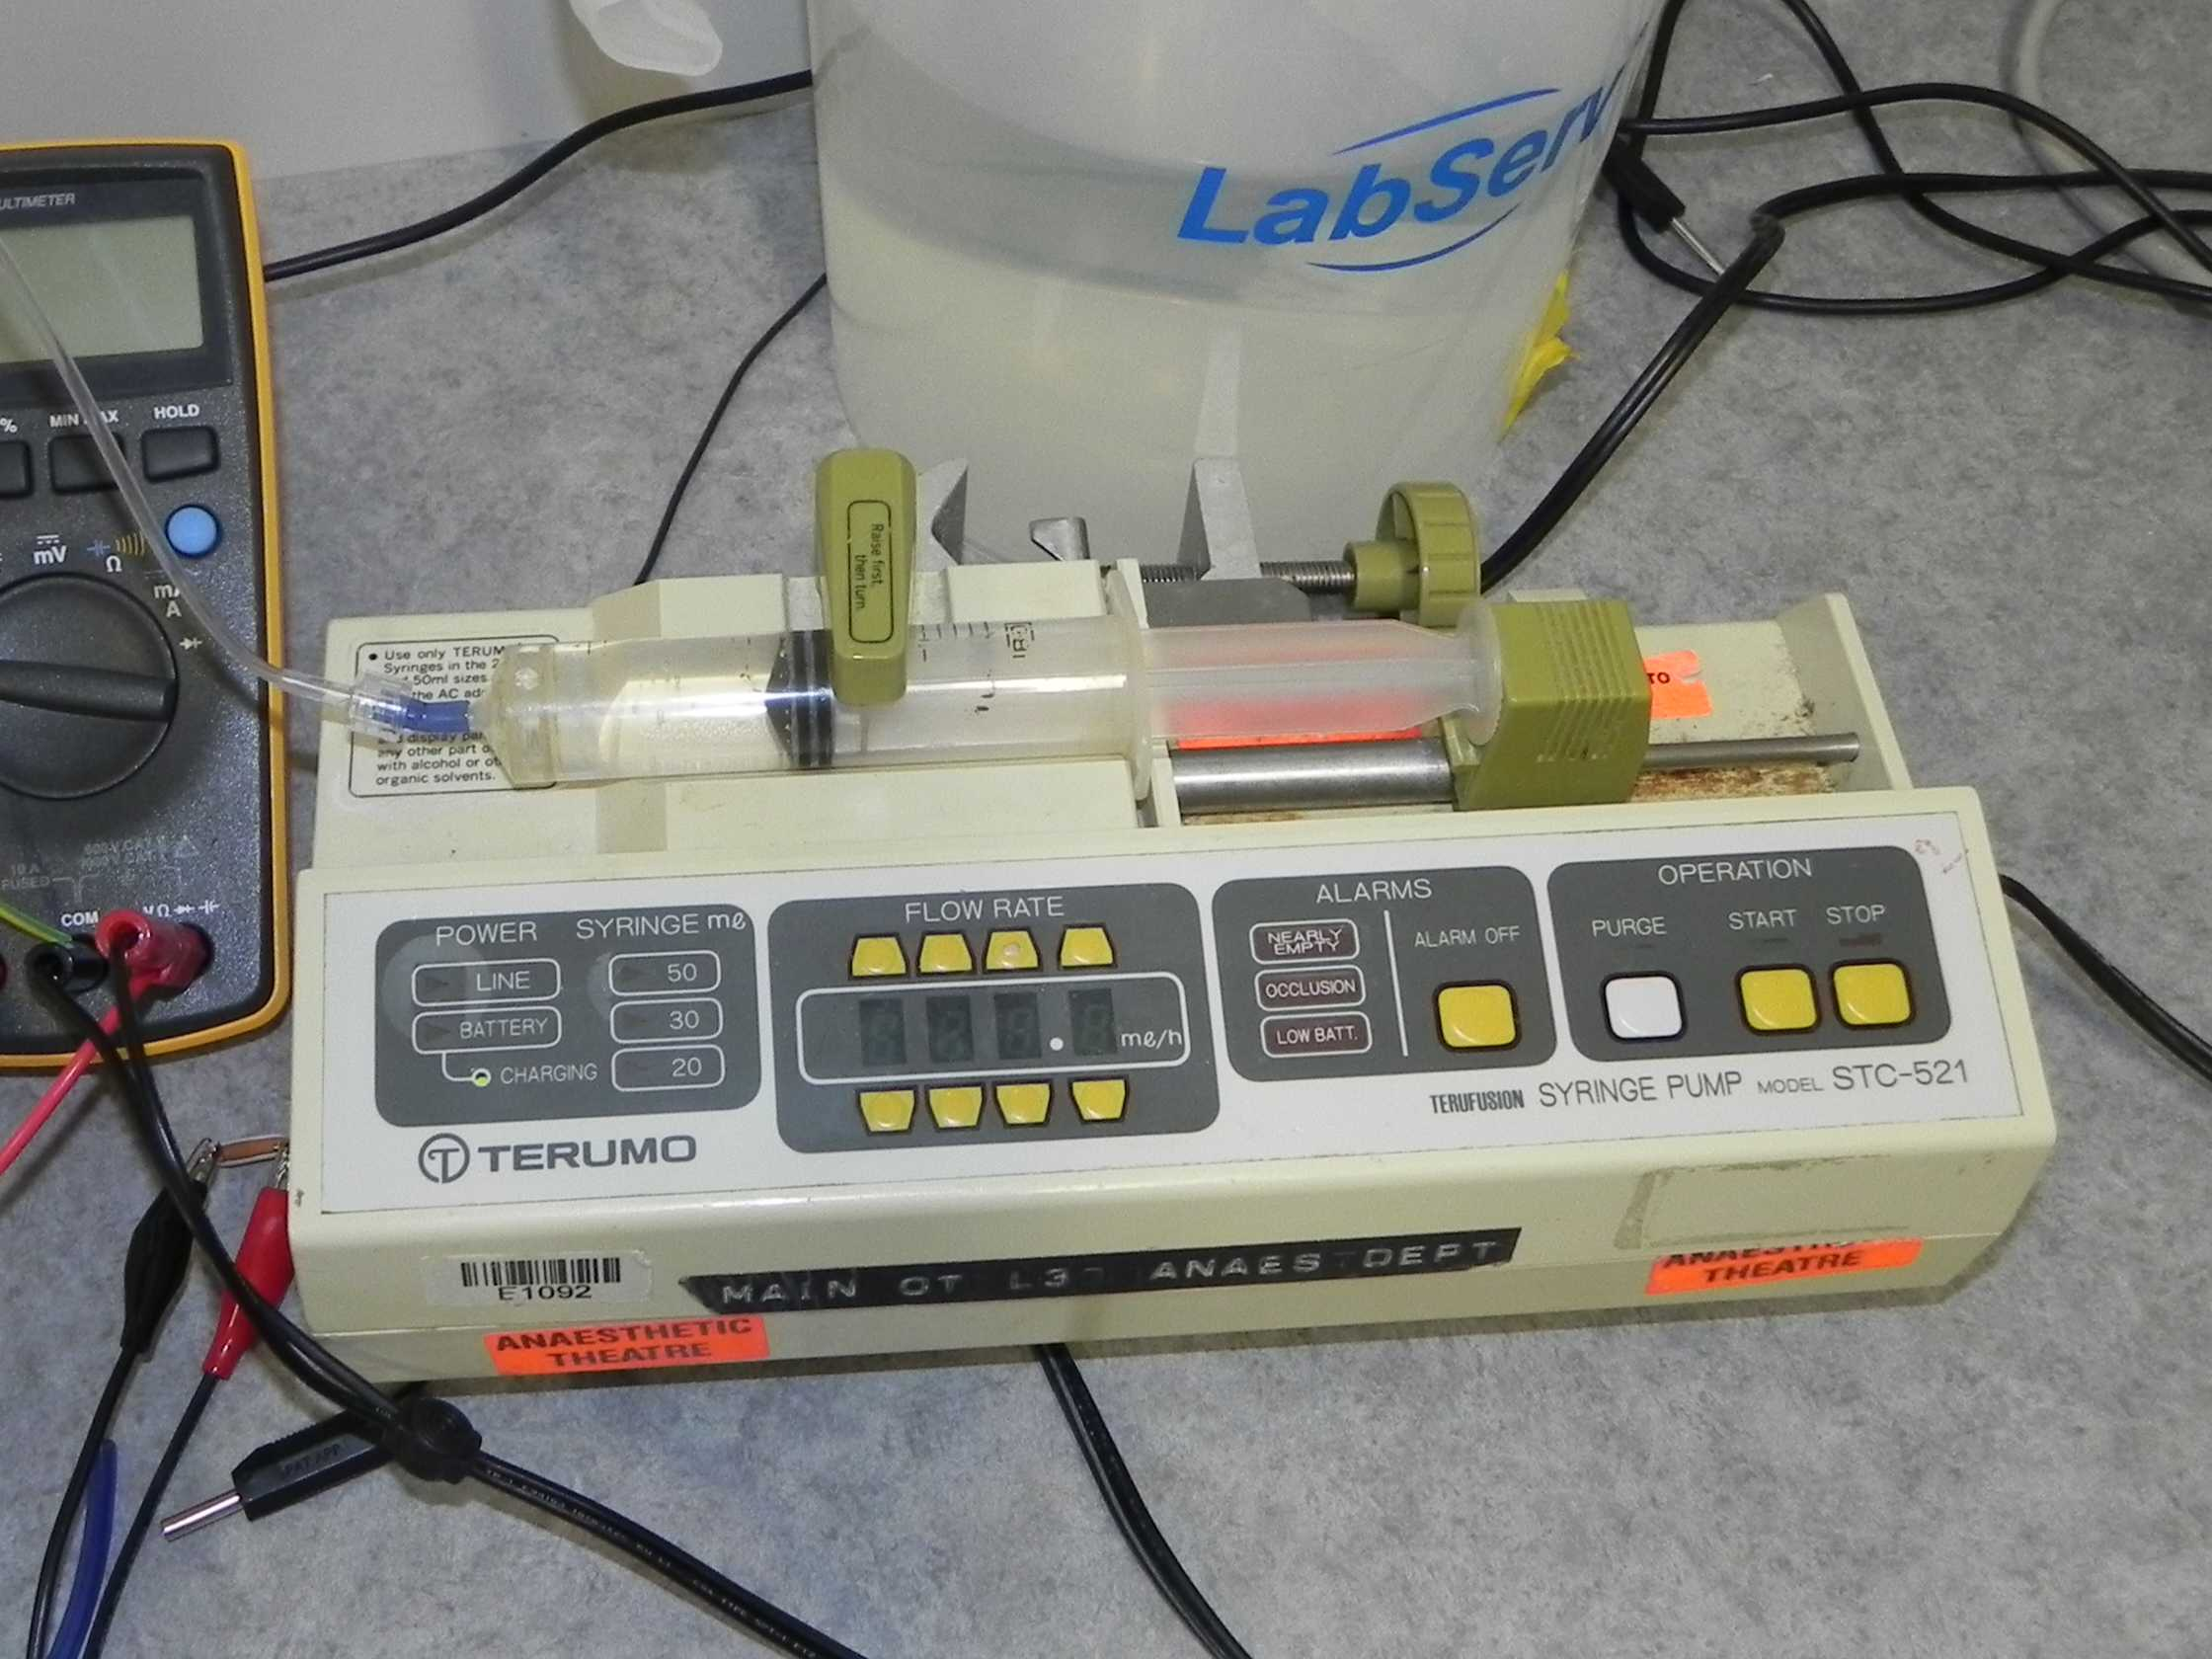
\includegraphics[scale=0.15]{content/appendices/chargedWaterDrops/graphics/Photo_dripperExperiment_SyringePump_draft.JPG}
    \caption{\label{Photo_dripperExperiment_SyringePump}Syringe pump used to produce drops and control flow rate.}
\end{figure}

\subsubsection*{Results}

\begin{figure}
    \centering
    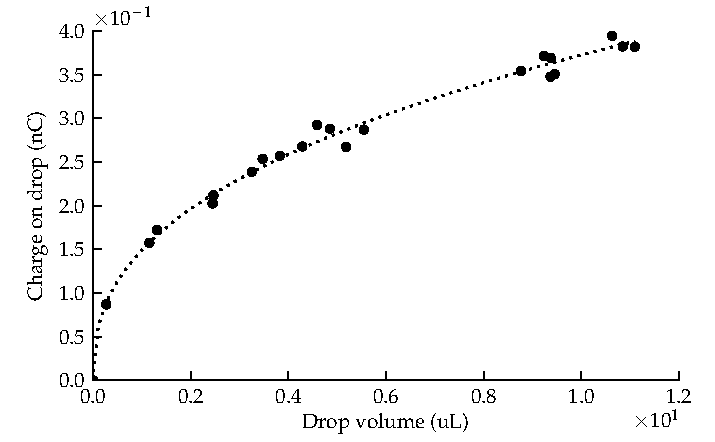
\includegraphics{content/appendices/chargedWaterDrops/graphics/dripper_chargeVsVolume}
    \caption{\label{Graph_dripperExperiment_chargeVsVolume}Charge on drip versus drip volume for a fixed induction voltage of \SI{2.5}{\kilo\volt}.}
\end{figure}
Figure \ref{Graph_dripperExperiment_chargeVsVolume} shows the effect
that changing the volume of each drop has on the amount of charge
bound to that drop. The shape of this curve is similar to what one
gets when plotting the surface area of a sphere against the volume
of a sphere. This was expected to be the case since excess charge
will position itself evenly over the surface of the drop and hence
be proportional to its surface area. If the same data is plotted in
terms of charge per volume versus volume of a drip, as is shown in
Figure \ref{Figure_Graph_dripper_chargePerVolumeVsVolume}, it is
evident that smaller drop sizes equate to a higher charge per volume
of water ratio.

\begin{figure}
    \centering
    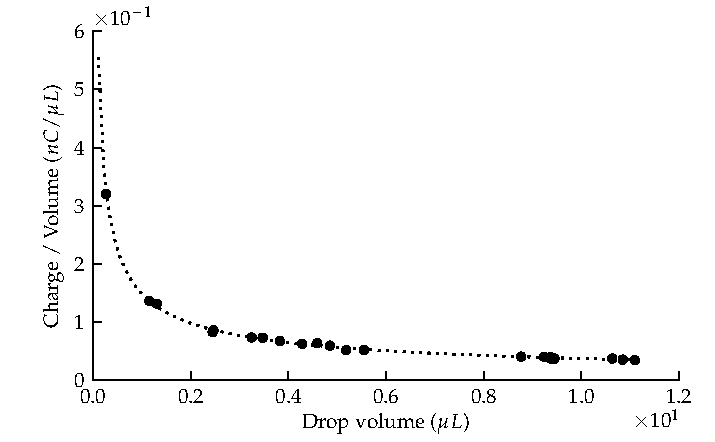
\includegraphics{content/appendices/chargedWaterDrops/graphics/dripper_chargePerVolumeVsVolume}
    \caption{\label{Figure_Graph_dripper_chargePerVolumeVsVolume}Charge per volume
    versus drop volume for a fixed induction voltage of \SI{2.5}{\kilo\volt}.}
\end{figure}


Figure \ref{Figure_Graph_dripper_chargeVsVoltage} shows the results
of changing the induction voltage on the average charge carried per
drop. These results indicate that the charge induced on a drop is
proportional to the induction voltage. Variation in the measurement
data was due to differences in room temperature.

\begin{figure}
    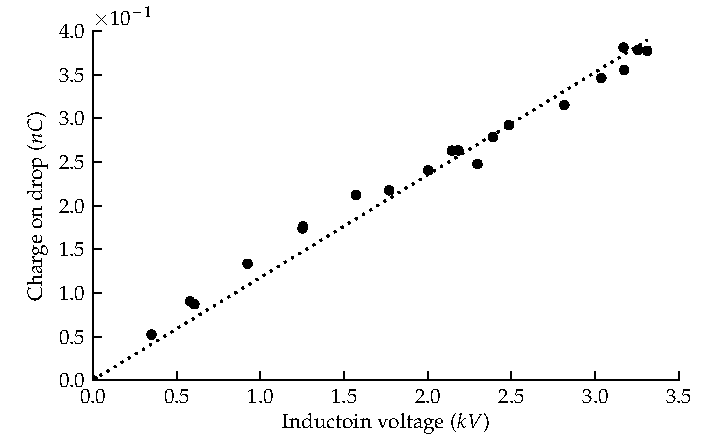
\includegraphics{content/appendices/chargedWaterDrops/graphics/dripper_chargeVsVoltage}
    \caption{\label{Figure_Graph_dripper_chargeVsVoltage}Charge on drip versus ring induction voltage for a fixed drip volume.}
\end{figure}


Figure \ref{Figure_Graph_dripper_currentVsFlow} shows the effect
of increasing the flow on the output current of the measurement setup,
which is relatively linear.

\begin{figure}
    \centering
    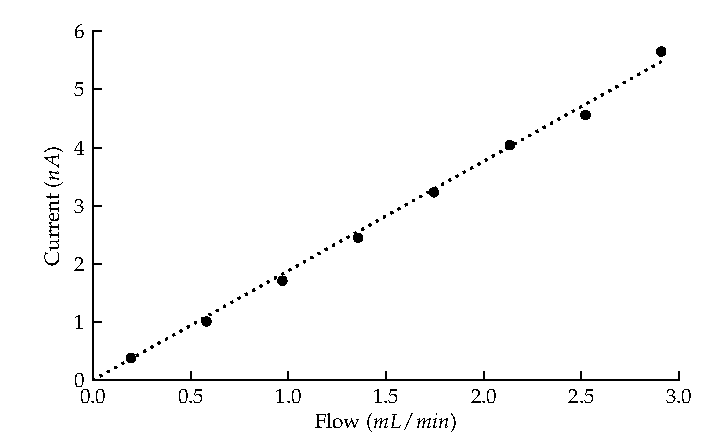
\includegraphics{content/appendices/chargedWaterDrops/graphics/dripper_currentVsFlow}
    \caption{\label{Figure_Graph_dripper_currentVsFlow}Current versus flow rate
    for an induction voltage of \SI{3.8}{\kilo\volt} and drop volume of \SI{3.1}{\micro\litre}.}
\end{figure}



\subsubsection*{Conclusion \& discussion}

Increasing the output of the initial apparatus is possible by doing
any of the following things:
\begin{itemize}
\item Favour smaller drops at higher frequencies.
\item Increase the total flow of water through the apparatus.
\item Increase the induction voltage.
\end{itemize}
Increasing the total flow through the apparatus is difficult to achieve
as this soon has adverse effects on the formation of drops. This usually
leads to the formation of a stream of water from the needle, reducing
the output as the drips aren't forming within the inductor.

Favouring small drops or increasing the induction voltage both increase
the charge to mass ratio of individual drops. As this ratio increases
the movement of the drops becomes increasingly dominated by electrostatic
forces between the container and the drop. As this ratio increases
so to does the tendency for drops to diverge from the path dictated
by gravity. Eventually there comes a point where the drops no-longer
fall and instead create a stream that loops to the nearest point on
the induction ring. For this reason it is important that drop sizes
are kept consistent as to maintain a stable charge to mass ratio to
which the design can be optimised for.


\subsection*{Scale}

Due to the size of the apparatus the fields generated had to be relatively
large, requiring equally large voltages before useful amounts of power
is generated. There are two problems with generating power at such
large voltages:
\begin{enumerate}
\item Large voltage differences try very hard to neutralise each other.
This means that the geometry and materials used may need to be modified
in order to reduce charge migrating over insulating barriers.
\item Stepping these voltages down to a useful level is challenging and
would be very inefficient. Electronic components and configurations
that would usually be used to change voltage levels no longer work.
\end{enumerate}
Scaling down the design would allow the device to generate its maximum
practical output at voltages that are easier to deal with.


\subsubsection*{Investigation:}

\begin{figure}
    \centering
    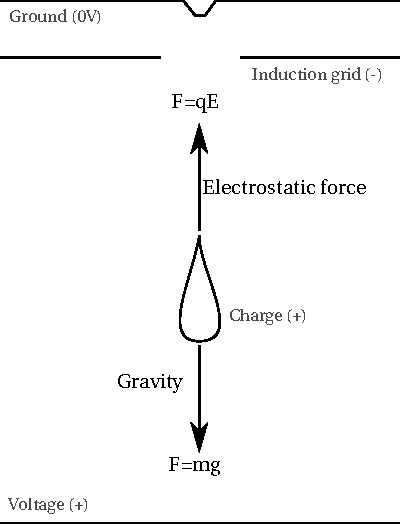
\includegraphics{content/appendices/chargedWaterDrops/graphics/ChargedDrips_Figure_Diagram_Forces}
    \caption{\label{Figure_Diagram_ChargedDrips_Figure_Diagram_Forces}Diagram
of the electrostatic force and gravity acting on a drop of water.}
\end{figure}


Figure \ref{Figure_Diagram_ChargedDrips_Figure_Diagram_Forces} shows
a simplified diagram of the two dominant forces acting upon a charged
drop as it falls towards a like charged plate from a grounded plane.
These two forces are given by the following equations:

\begin{equation}
F_{down}=mg
\end{equation}


\begin{equation}
F_{up}=qE
\end{equation}


Where $m$ is the mass of the drop, $g$ is the acceleration due to
gravity, $q$ is the charge on the drop and $E$ is the electric field
strength.
